\documentclass[aspectratio=169]{beamer}

%
% Choose how your presentation looks.
%
% For more themes, color themes and font themes, see:
% http://deic.uab.es/~iblanes/beamer_gallery/index_by_theme.html
%
\mode<presentation>
{
  \usetheme{default}      % or try Darmstadt, Madrid, Warsaw, ...
  \usecolortheme{default} % or try albatross, beaver, crane, ...
  \usefonttheme{default}  % or try serif, structurebold, ...
  \setbeamertemplate{navigation symbols}{}
  \setbeamertemplate{caption}[numbered]
  \setbeamertemplate{footline}[page number]
  \setbeamercolor{frametitle}{fg=white}
  \setbeamercolor{footline}{fg=black}
} 

\usepackage[english]{babel}
\usepackage[utf8x]{inputenc}
\usepackage{tikz}
\usepackage{listings}
\usepackage{courier}

\xdefinecolor{darkblue}{rgb}{0.1,0.1,0.7}
\xdefinecolor{dianablue}{rgb}{0.18,0.24,0.31}
\definecolor{commentgreen}{rgb}{0,0.6,0}
\definecolor{stringmauve}{rgb}{0.58,0,0.82}

\lstset{ %
  backgroundcolor=\color{white},      % choose the background color
  basicstyle=\ttfamily\small,         % size of fonts used for the code
  breaklines=true,                    % automatic line breaking only at whitespace
  captionpos=b,                       % sets the caption-position to bottom
  commentstyle=\color{commentgreen},  % comment style
  escapeinside={\%*}{*)},             % if you want to add LaTeX within your code
  keywordstyle=\color{blue},          % keyword style
  stringstyle=\color{stringmauve},    % string literal style
  showstringspaces=false,
  showlines=true
}

\lstdefinelanguage{scala}{
  morekeywords={abstract,case,catch,class,def,%
    do,else,extends,false,final,finally,%
    for,if,implicit,import,match,mixin,%
    new,null,object,override,package,%
    private,protected,requires,return,sealed,%
    super,this,throw,trait,true,try,%
    type,val,var,while,with,yield},
  otherkeywords={=>,<-,<\%,<:,>:,\#,@},
  sensitive=true,
  morecomment=[l]{//},
  morecomment=[n]{/*}{*/},
  morestring=[b]",
  morestring=[b]',
  morestring=[b]"""
}

\title[2016-09-15-strangeloop]{\sc \large \textcolor{black}{making histograms functional}}
\author{\textcolor{darkblue}{Jim Pivarski}}
\institute{\textcolor{darkblue}{Princeton University -- DIANA-HEP}}
\date{\textcolor{darkblue}{September 15, 2016}}

\begin{document}

\logo{\pgfputat{\pgfxy(0.11, 7.4)}{\pgfbox[right,base]{\tikz{\filldraw[fill=dianablue, draw=none] (0 cm, 0 cm) rectangle (50 cm, 1 cm);}
\includegraphics[height=1 cm]{diana-hep-logo.png}}}}

\begin{frame}
  \vspace{1.25 cm}
  \begin{center}
    
\includegraphics[width=0.6\linewidth]{histogrammar-logo.png}
  \end{center}

  \vspace{-1.25 cm}
  \titlepage
\end{frame}

% Uncomment these lines for an automatically generated outline.
%\begin{frame}{Outline}
%  \tableofcontents
%\end{frame}

\begin{frame}{Tale of two cities}
\vspace{0.2 cm}
\begin{columns}
\column{0.5\linewidth}
\begin{center}
\textcolor{darkblue}{\Large \underline{Statistical Computing}}

\vspace{0.25 cm}
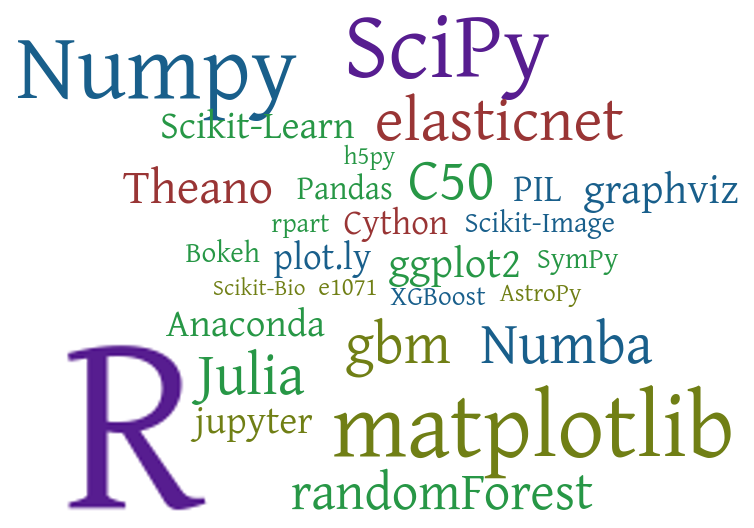
\includegraphics[height=3.5 cm]{statistical-software.png}
\end{center}

\begin{onlyenv}<2->
\begin{itemize}
\item Often natively compiled, driven by high-level languages.
\item Primary customer is the laptop data analysis.
\end{itemize}
\end{onlyenv}

\column{0.5\linewidth}
\begin{center}
\textcolor{darkblue}{\Large \underline{Big Data}}

\vspace{0.25 cm}
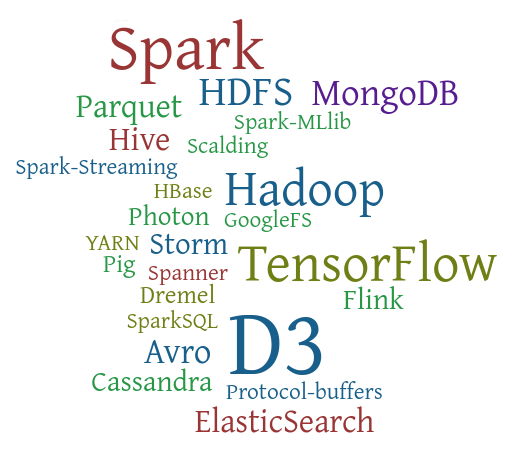
\includegraphics[height=3.5 cm]{bigdata-software.png}
\end{center}

\begin{onlyenv}<2->
\begin{itemize}
\item Usually Java/Spark/Clojure.
\item More emphasis on scale-out than single-processor speed.
\item Datasets assumed to be {\it big.}
\end{itemize}
\end{onlyenv}

\end{columns}
\end{frame}

\begin{frame}{A third you may not have heard about}
\vspace{0.5 cm}
\begin{center}
\textcolor{darkblue}{\Large \underline{High Energy Physics (HEP)}}

\vspace{0.25 cm}
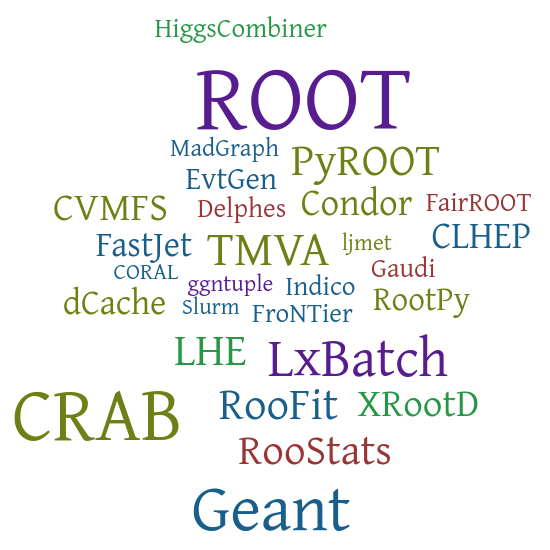
\includegraphics[height=6 cm]{hep-software.png}
\end{center}
\end{frame}

\begin{frame}{A third you may not have heard about}
\vspace{0.25 cm}
\begin{columns}
\column{0.5\linewidth}
\begin{center}
\textcolor{darkblue}{\Large \underline{High Energy Physics (HEP)}}

\vspace{0.25 cm}
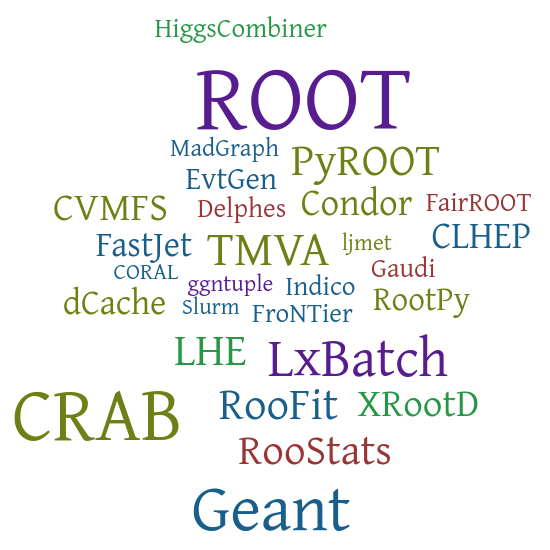
\includegraphics[height=6 cm]{hep-software.png}
\end{center}

\column{0.5\linewidth}
\begin{itemize}
\item Natively compiled, optimized for single-processor throughput.
\item<2-> {\it Throughput,} not speed, this is not High Performance Computing (HPC).
\item<3-> Datasets have always been ``big'' 
\begin{itemize}
\item<4-> SPS in 1980's: $\sim$100~GB per year
% https://www.researchgate.net/publication/275209564_UA1_Data-acquisition_System 1.6 MB/event? (``raw'')
% https://cern.ch/delfino/Generic%20LHC%20Computing%202000.ppt 0.1 MB/event (probably after processing)
% http://cerncourier.com/cws/article/cern/28849
\item<5-> LHC today: $\sim$25~PB per year
% http://www.lhc-closer.es/taking_a_closer_look_at_lhc/0.lhc_data_analysis
% https://home.cern/about/updates/2013/02/cern-data-centre-passes-100-petabytes
\end{itemize}
\end{itemize}

\vspace{0.2 cm}
\hfill \only<6>{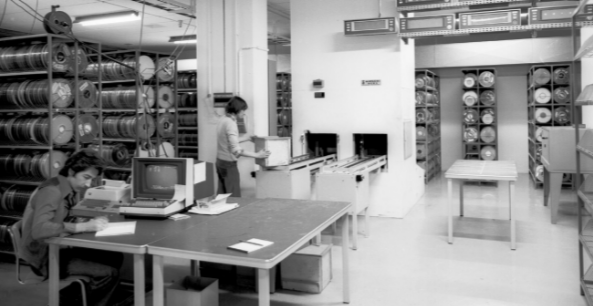
\includegraphics[width=0.87\linewidth]{tapes1.png}}\only<7>{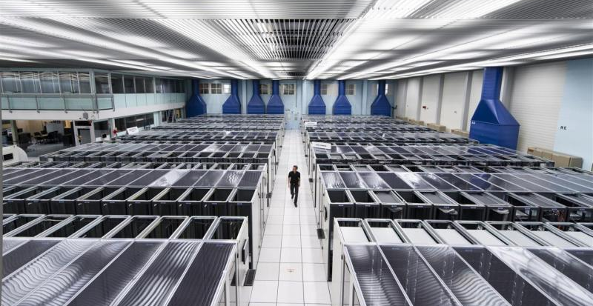
\includegraphics[width=0.87\linewidth]{cerncomputing.png}}
\vspace{-0.2 cm}
\end{columns}
\end{frame}

%% \begin{frame}{A third you may not have heard about}
%% \vspace{0.5 cm}
%% \begin{columns}
%% \column{0.5\linewdith}
%% \begin{center}
%% \textcolor{darkblue}{\Large \underline{High Energy Physics (HEP)}}

%% \vspace{0.25 cm}
%% 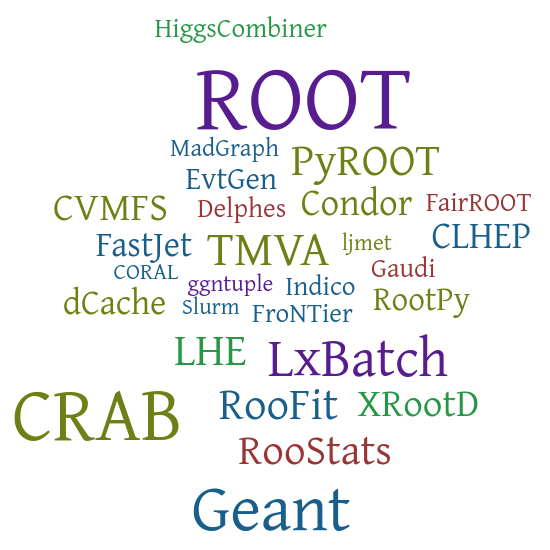
\includegraphics[height=6 cm]{hep-software.png}
%% \end{center}

%% \column{0.5\linewdith}
%% \begin{itemize}
%% \item 
%% \end{itemize}
%% \end{columns}
%% \end{frame}


\end{document}
